\documentclass[a4paper,11pt]{article}
\usepackage{graphicx}
\usepackage{booktabs}
\usepackage{siunitx}

\setlength{\voffset}{-25mm}
\setlength{\hoffset}{-10mm}
\setlength{\oddsidemargin}{0mm}
\setlength{\evensidemargin}{0mm}

\setlength{\marginparwidth}{0mm}
\addtolength{\textwidth}{45mm}
\addtolength{\textheight}{55mm}

\begin{document}
\begin{figure}
	\centering
	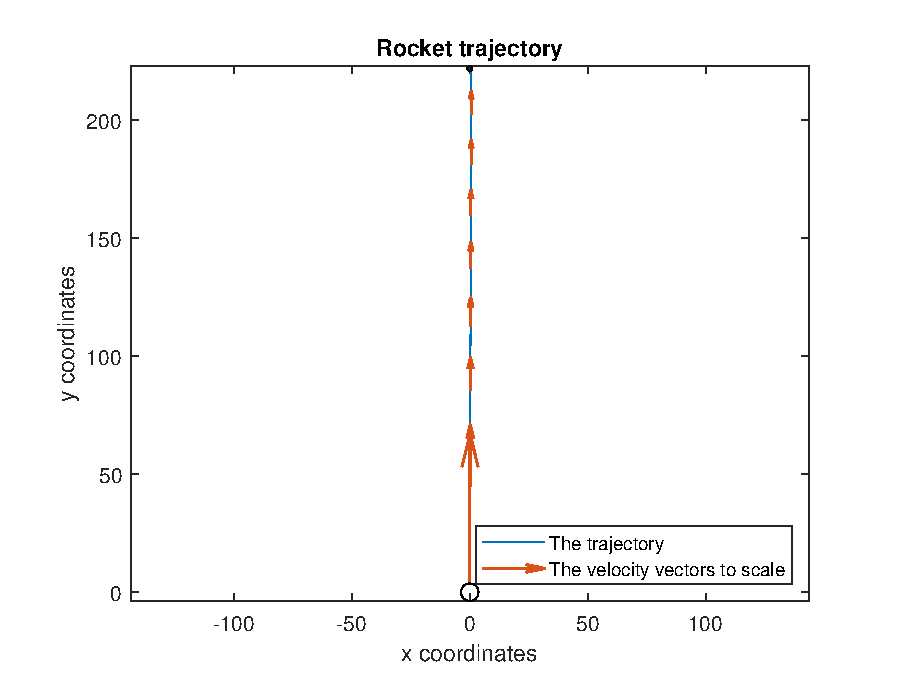
\includegraphics[width=\textwidth]{stationary1}
\end{figure}
\begin{figure}
	\centering
	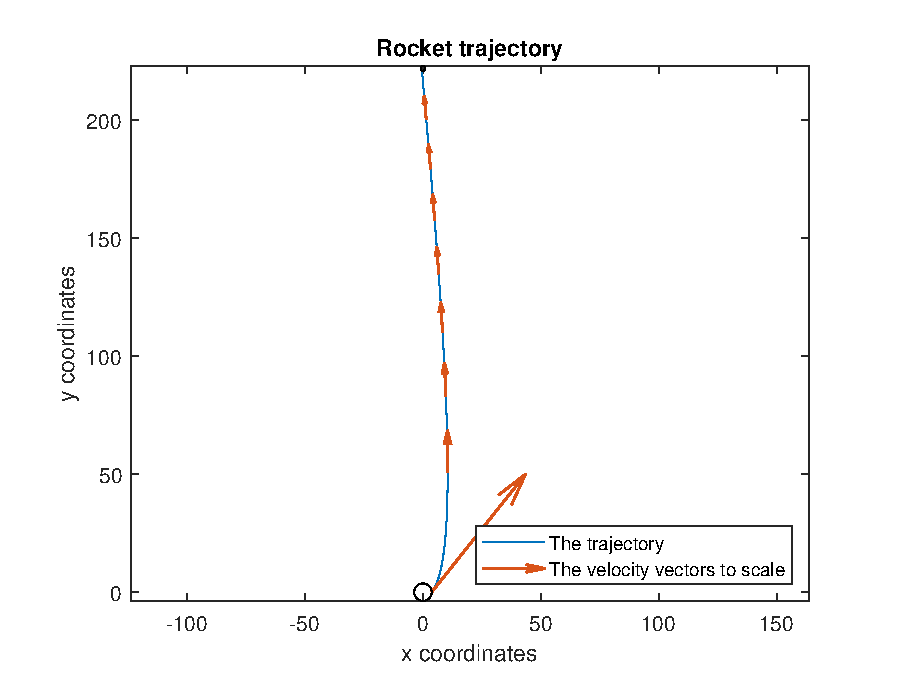
\includegraphics[width=\textwidth]{stationary2}
\end{figure}
\begin{figure}
	\centering
	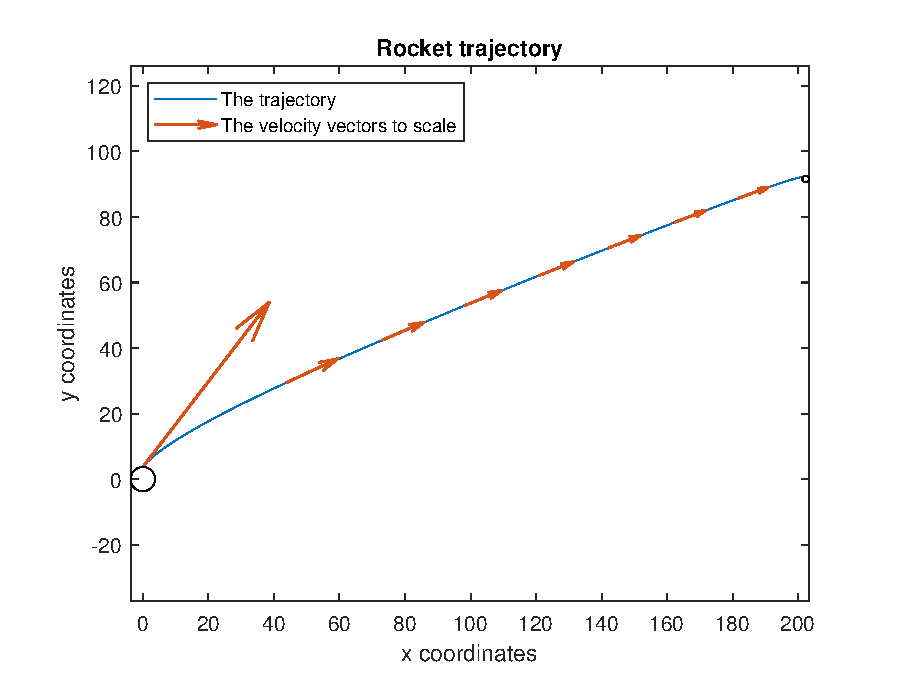
\includegraphics[width=\textwidth]{moving}
\end{figure}
\begin{figure}
	\centering
	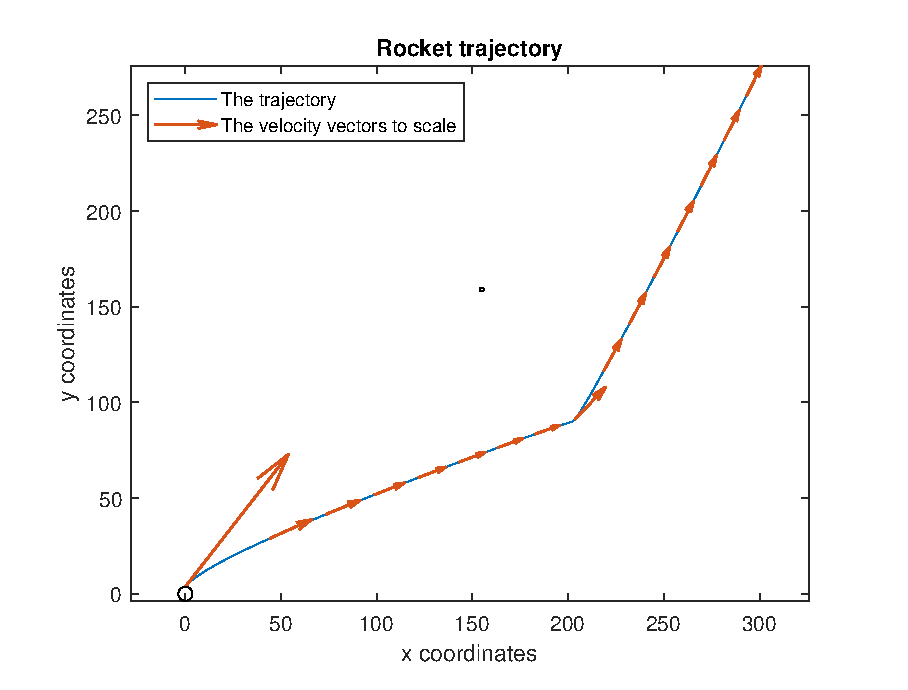
\includegraphics[width=\textwidth]{slingshot}
\end{figure}
\begin{table}
	\centering
	\sisetup{table-number-alignment=center}
	\begin{tabular}{
			S[table-figures-integer = 2, table-figures-decimal=0]
			S[
				table-figures-integer = 1,
				table-figures-decimal = 6
			]
			S[
				table-figures-integer = 1,
				table-figures-decimal = 3
			]
		}
		\toprule
		{m, \si{g}} & {$\tau$, \si{N.m}} & {$\theta$, \si{rad}} \\
		\midrule
		0 & 0.000000 & 0.000 \\
		20 & 0.004681 & 1.670 \\
		40 & 0.009363 & 3.616 \\
		50 & 0.011703 & 4.494 \\
		60 & 0.014044 & 5.397 \\
		70 & 0.016385 & 6.240 \\
		80 & 0.018725 & 7.570 \\
		90 & 0.021066 & 9.484 \\
		\bottomrule
	\end{tabular}
\end{table}
\begin{table}
	\caption{Aligning the \texttt{S} column.}
	\label{tab:S:align}
	\centering
	\sisetup{
		table-figures-integer = 2,
		table-figures-decimal = 4
	}
	\begin{tabular}{
			S
			S[table-number-alignment = center]
			S[table-number-alignment = left]
			S[table-number-alignment = right]
		}
		\toprule
		{Some Values} & {Some Values} & {Some Values} & {Some Values} \\
		\midrule
		2.3456 & 2.3456 & 2.3456 & 2.34562131 \\
		34.2345 & 34.2345 & 34.2345 & 34.2345 \\
		56.7835 & 56.7835 & 56.7835 & 56.7835 \\
		90.473 & 90.473 & 90.473 & 90.473 \\
		\bottomrule
	\end{tabular}
\end{table}

\end{document}